\subsection{DQ Alignment}

The DQalign interface works in a manner similar to that described by
XAPP701. We measure the position of the DQS strobe during a burst-read
cycle by varying the input delay and looking for edge transitions.

Then we properly advance the IDELAY associated with the data registers. 

We begin the measurement cycle by asserting START at the
rough-beginning of a burst-read, which will read out 512 words. The
increment-delay-measure cycle should take <5 ticks so we should have
time to make a full sweep during the single burst.

\begin{figure}
\begin{centering}
\includegraphics[scale=0.8]{dqalign.svg}
\end{centering}
\caption{DQS and Data Alignment Interface }
\label{dqalign}
\end{figure}

\begin{figure}
\begin{centering}
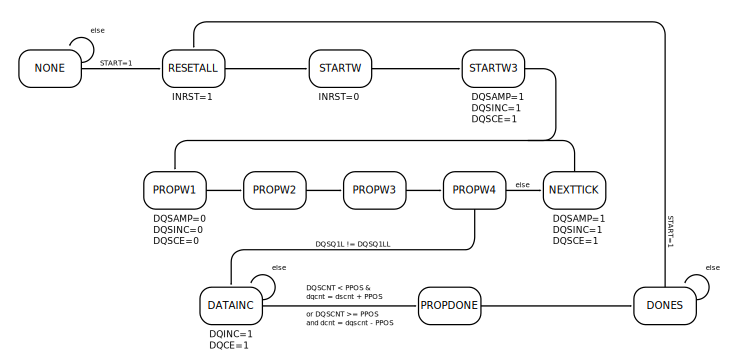
\includegraphics[scale=0.8]{dqalign.fsm.svg}
\end{centering}
\caption{DQS and Data Alignment Interface FSM.}
\label{dqalign}
\end{figure}

